\section{Evaluation}
\label{evaluation}
Now that we have shown the design, implementation, and application of our advert
server, we would like to evaluate its performance. More specific; how does the
system behaves under various circumstances? Therefore, we designed a couple of
benchmarks to measure its performance, expressed in completion time, latency,
and bandwidth.

Before starting our benchmarks, we used the UNIX \texttt{traceroute} command to
determine where our App Engine application is hosted. The results can be found in
Figure \ref{tracert}. The last known IP address resides at Mountain View,
California (US), which is where Google Inc. is residing. It is safe to assume
that all our request go to Google US and back.

\begin{figure*}[h,b] %[placement] where placement is h,t,b,p
\begin{center}
\begin{code}
$ traceroute ibisadvert.appspot.com
traceroute to appspot.l.google.com (74.125.79.141), 64 hops max, 40 byte packets
 1  router-student1 (130.37.24.7)  0.641 ms  0.314 ms  0.293 ms
 2  hkae16-2-d02.backbone.vu.nl (130.37.5.54)  0.288 ms  0.257 ms  0.274 ms
 3  GE5-1-1.2090.JNR01.Asd002A.surf.net (145.145.20.57)  0.674 ms  0.665 ms  0.620 ms
 4  AE0.500.JNR02.Asd002A.surf.net (145.145.80.65)  0.690 ms  0.657 ms  0.745 ms
 5  core1.ams.net.google.com (195.69.144.247)  1.156 ms  0.993 ms  0.997 ms
 6  209.85.248.93  11.159 ms  1.353 ms  1.269 ms
 7  64.233.175.246  14.791 ms 72.14.233.114  6.209 ms 64.233.175.246  4.269 ms
 8  72.14.239.199  5.749 ms 209.85.255.166  5.932 ms 72.14.239.197  4.606 ms
 9  209.85.255.126  7.864 ms 209.85.255.122  6.025 ms  6.676 ms
 10  * * *
\end{code}
\caption{Traceroute output of ibisadvert.appspot.com.\label{tracert}}
\end{center}
\end{figure*}

\subsection{Benchmarks}
The benchmarks designed can be divided in three categorees: completion time of
client and server functions, bandwidth, and parallel benchmarks. All measurements
below were perfomed on a 2.16\,GHz Intel Core 2 Duo iMac, with 1\,GB 667\,MHz
DDR2 SDRAM. Network performance may vary, depending on your bandwidth and network
traffic. We did our measurements from the \emph{Vrije Universiteit}, which owns a
fibreglass internet connection provided by \emph{SURFnet}. For or parallel
benchmarks we made use of the VU's \emph{DAS-3 cluster}, which has 85 dual-core
2.4\,GHz nodes, with 4\,GB of memory and a Myri-10G and GbE network \cite{das3-www}.

\subsubsection{Completion Time}
To measure our performance we first of all will measure the completion time of
various parts of the system. The completion time will be measured client-side
and server-side (if relevant and possible), whilst sending and receiving
different amounts of data to and from the server. 

We will measure each client function individually, as well as starting up the
client library (authentication). The client and server functions which we are
most interested in are \texttt{add()}, \texttt{get()}, \texttt{delete()}, and
\texttt{find()}. All functions will be started with different amounts of 
data, ranging from 730\,bytes, to 730\,000\,bytes (since we still have to encode
everything in Base64, the actual data being sent ranges from 1\,kB to 1\,000\,kB,
respectively, the latter being the maximum call size of the Google datastore
API). In addition, we will also send various number of meta data items to the
server, ranging from 0 to 1\,000 key-value pairs. Also we will test how long
the search for a particular data item in the datastore would take, if different
amounts of data are present in the datastore. These amounts range from 10 to
1\,000 items.

All measurements will be done with respect to the authenticated server (unless
stated otherwise), because we expect it will be used most in practice. We will
repeat every measurement 10 times, and take the minimum, average, and maximum
from the set of completion times. Where applicable, we will also look at
individual completion times of various function components.

\subsubsection{Bandwidth}
In addition to the completion time, we will benchmark the bandwidth between the
Vrije Universiteit, Amsterdam, and the Google App Engine (located as stated in
Figure \ref{tracert}). To get an idea of the latency, we will first measure the
round trip delay, which is done by setting up a dummy server, which just
instantly sends a response as soon as it receives a request. 

Second, we will measure our upload speed by sending the maximum request size
(10\,MB according to Google) to the server, and have the server responding instantly.
Finally we will measure our download speed by requesting the maximum response
size (also 10\,MB).

\subsubsection{Parallel}
Last, we would like to know how the server performs if multiple clients would
connect at the same time. To test this, we used the Vrije Universiteit's DAS-3
cluster to spawn multiple clients at the same time. 

We will start a different number of clients simultaneously (ranging from 2 to 75
clients), and compare the completion time with the completion time of a single
client, doing the exact same operation. To ensure that all clients are doing
the same operation in parallel, we will repeat every operation ten times. All
measurements will be done client-side.

\subsection{Results}
Below we show the results of the measurements, as described above.

\subsubsection{Initialization}
Initializing our Advert library can be done in two different ways. First, we
have the public advert server, which does not require any authentication
whatsoever. Initializing this class takes a negligible amount of time (i.e.
less than 0ms).

Secondly, we have a private server model, which does require authentication.
Authenticating to a private advert server can be divided in three parts:

\begin{itemize}
  \item Authenticating to Google using ClientLogin
  \item Retrieving a authentication cookie from the Google App Engine
  \item Initializing and starting up `Persistent Authentication' thread
\end{itemize}

We measured the total time of initializing the Advert library (client-side),
which has an average of 190\,ms (179\,ms minimum, 229\,ms maximum). In addition
we measured each of the parts above individually, after which we can conclude
that authenticating using ClientLogin takes up one-third of the completion time
stated above, and retriving the authentication cookie takes up two-third of the
time measured above. Initializing and starting up our `Persistent Authentication'
thread takes a negligible amount of time (i.e. less than 1\,ms).

Note that it is impossible to measure server-side performance/completion time,
because ClientLogin and the process of retrieving a authentication cookie from the
Google App Engine, are both closed source procedures at Google, in which we
cannot place any timers.

\subsubsection{Add}
The process of adding an object to the datastore consists of four parts.

\begin{itemize}
  \item Processing the object (encoding to Base64 and JSON) and meta data
  \item Sending the object to the advert server
  \item Storing (possibly overwriting) the object and meta data
  \item Receiving a response
\end{itemize}

Below we state the results of the measurements we did client-side. Note that
the client-side measurements are network latency dependent, where the
server-side measurements are not (see Figures \ref{add-obj-size} and
\ref{add-md-size}).

\begin{figure} %[placement] where placement is h,t,b,p
\begin{center}
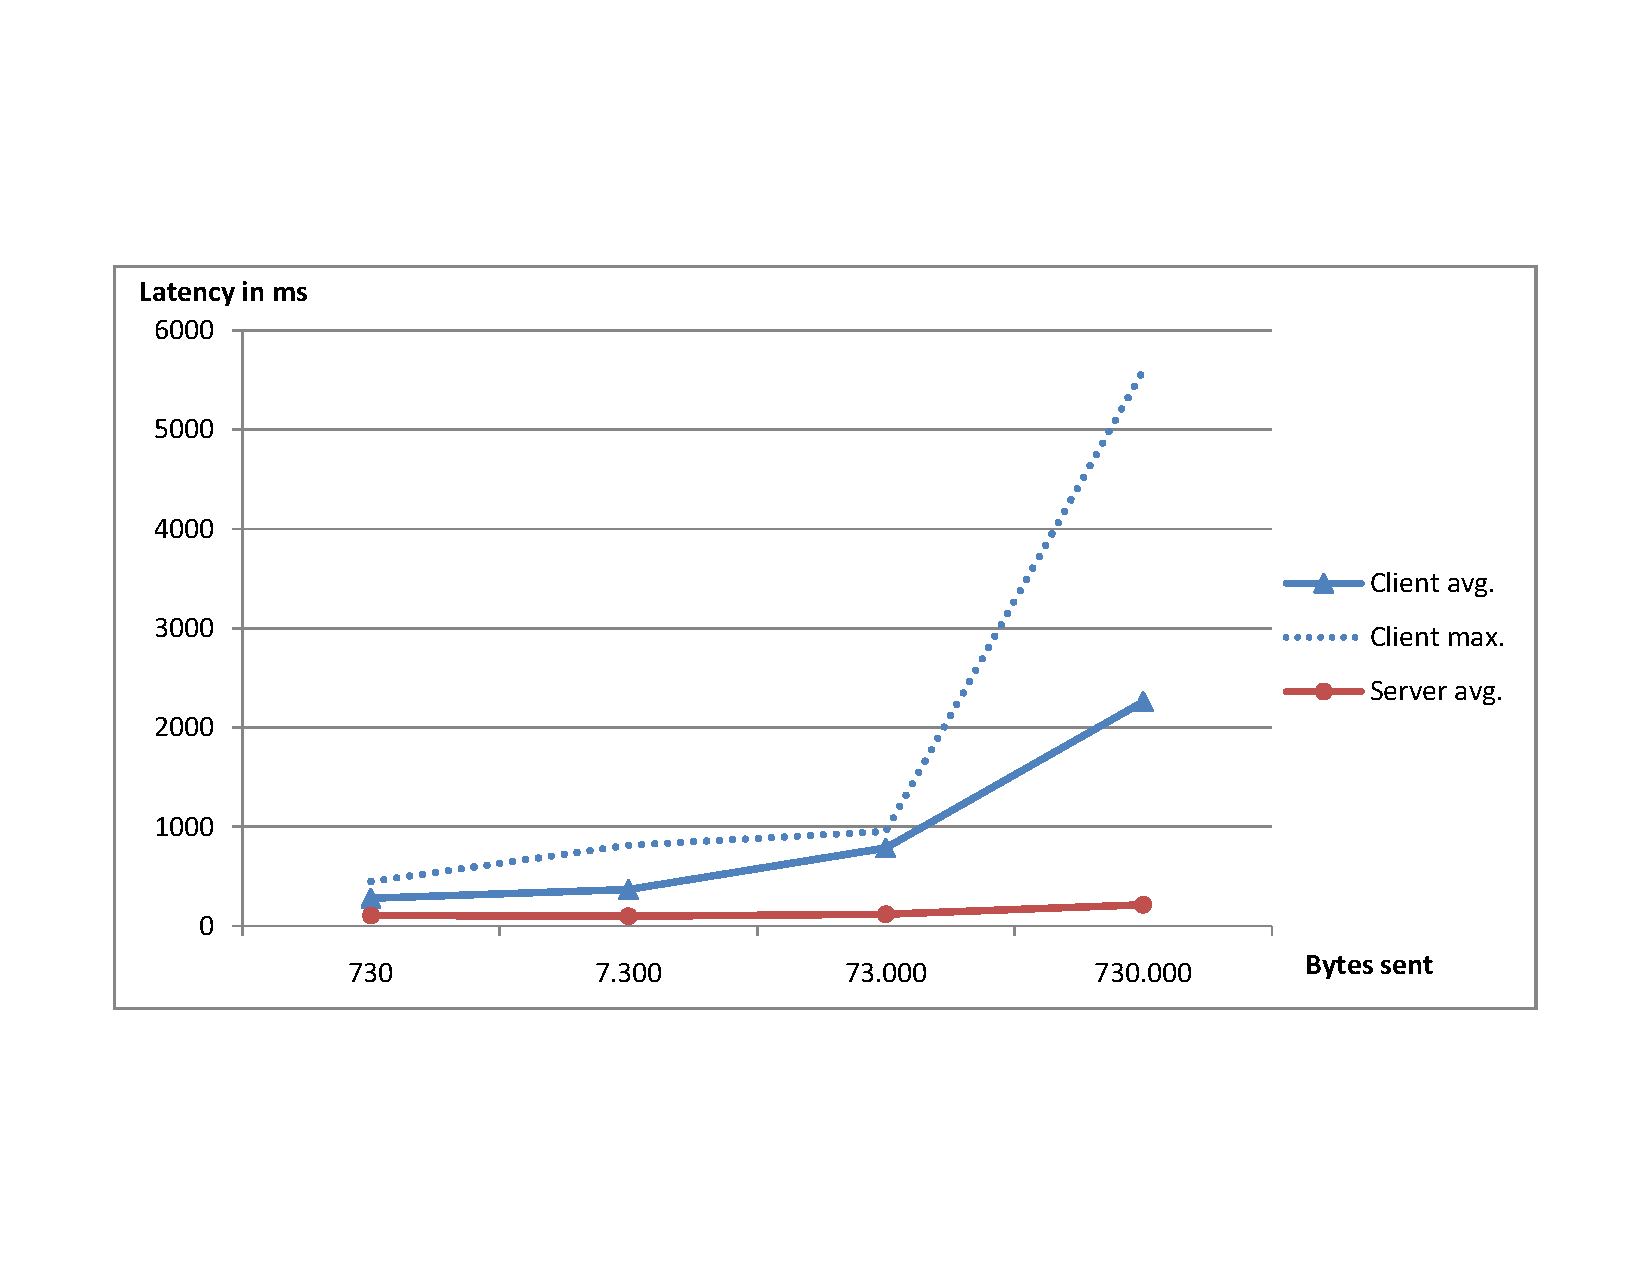
\includegraphics[trim=5cm 4cm 5cm 5cm,width=10cm]{./figures/add_obj.pdf}
\caption{Adding Objects of Variable Size. \label{add-obj-size}}
\end{center}
\end{figure}

\begin{figure} %[placement] where placement is h,t,b,p
\begin{center}
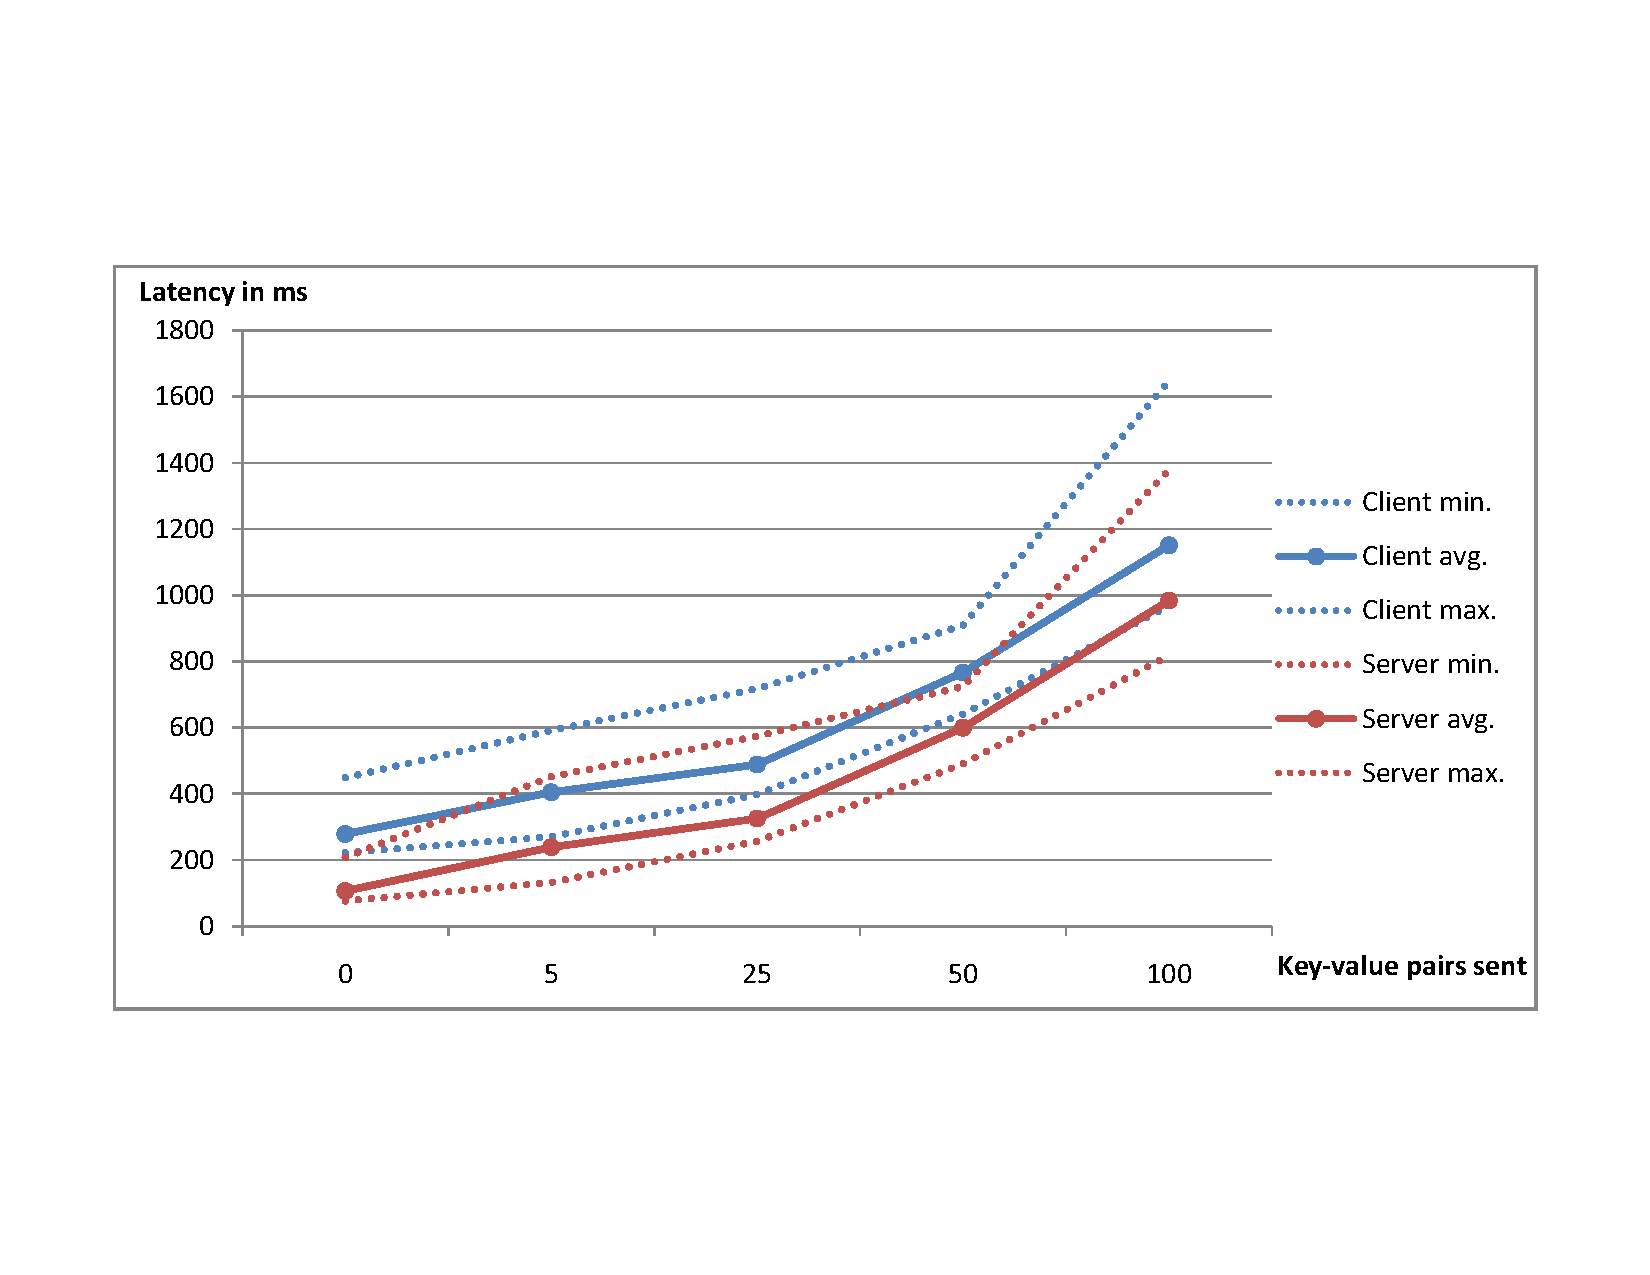
\includegraphics[trim=5cm 4cm 5cm 5cm,width=10cm]{./figures/add_md.pdf}
\caption{Adding Objects with Variable Meta Data. \label{add-md-size}}
\end{center}
\end{figure}

If we look at the subdivision of adding an object to the datastore, client side,
we see that for all results that encoding the data to Base64 takes a negligible
amount of time (less than 1\% of the total time, except when we add
730\,000\,bytes, this takes 2.6\% of the total time). Also the time to convert a
\texttt{MetaData} object to JSON takes a negligible amount of time (less than 1\%
of the total time), even when adding large numbers of key-value pairs (e.g. 100
pairs).

Note that two occasions can occur server-side: an entry does not exist yet; the
object is stored in the datstore. An object does already exits; the object is
overwritten. In the latter scenario, ideally, the maximum completion time would
not exceed the sum of the completion times of a \texttt{delete()} and an
\texttt{add()} statement (that is what overwrite does locally). The results of
our measurements can be found in Figures \ref{ovw-obj-size} and
\ref{ovw-md-size}.

\begin{figure} %[placement] where placement is h,t,b,p
\begin{center}
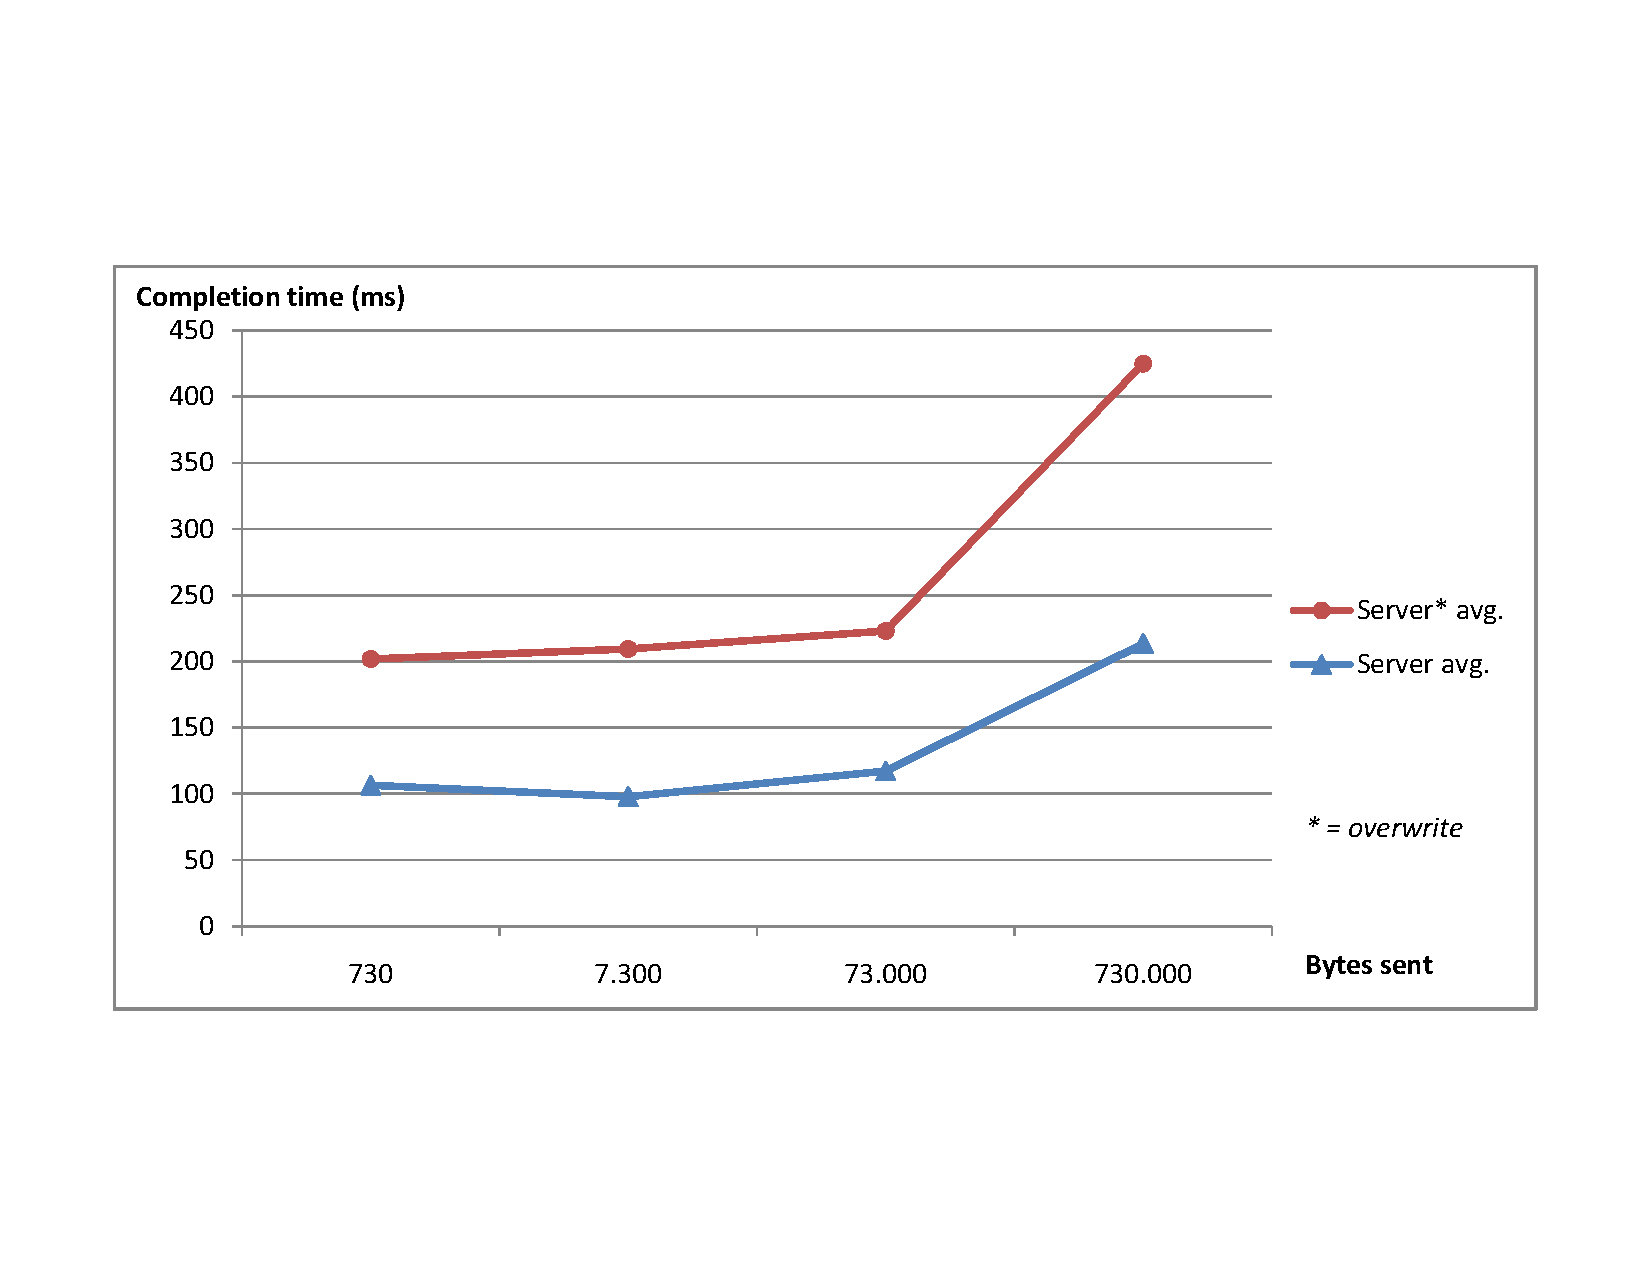
\includegraphics[trim=5cm 4cm 5cm 5cm,width=10cm]{./figures/ovw_obj.pdf}
\caption{Overwriting Objects of Variable Size. \label{ovw-obj-size}}
\end{center}
\end{figure}

\begin{figure} %[placement] where placement is h,t,b,p
\begin{center}
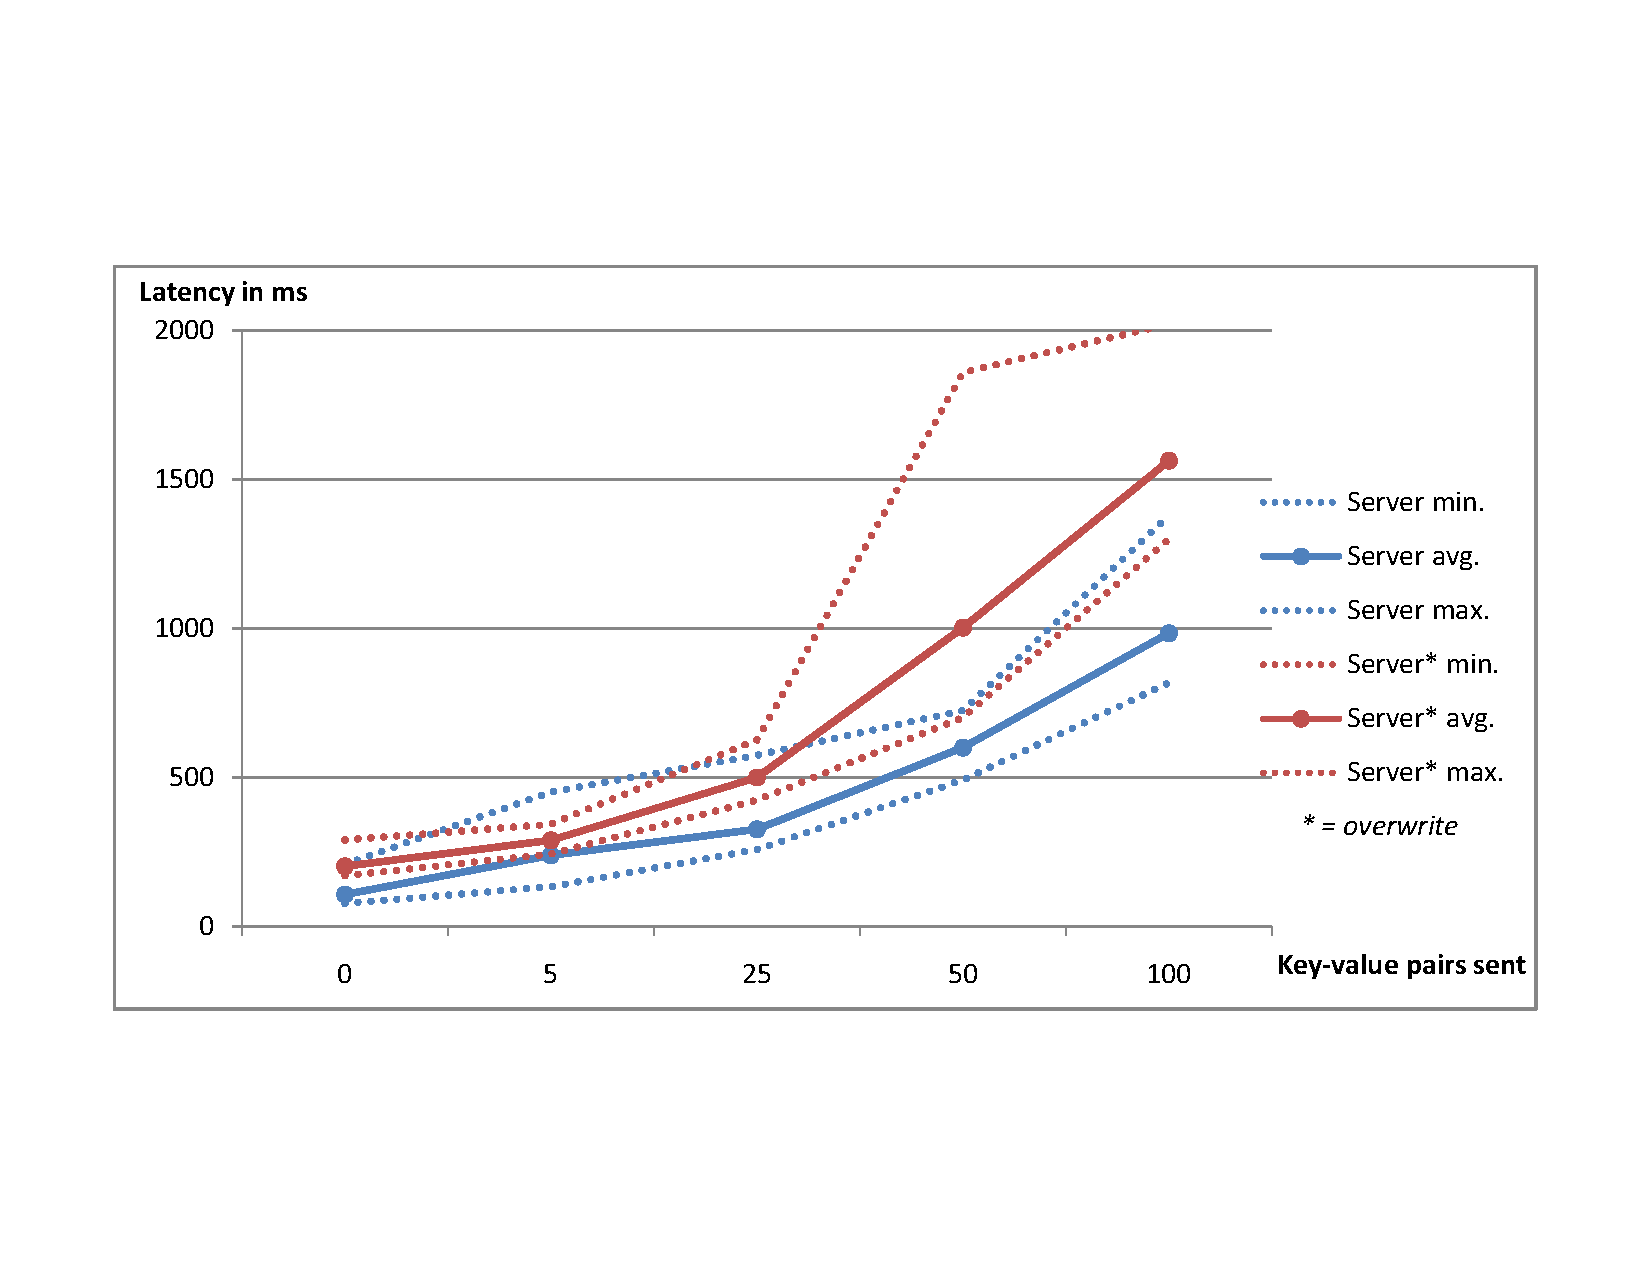
\includegraphics[trim=5cm 4cm 5cm 5cm,width=10cm]{./figures/ovw_md.pdf}
\caption{Overwriting Objects with Variable Meta Data. \label{ovw-md-size}}
\end{center}
\end{figure}

As expected, overwriting data takes more time than just adding data to the
datastore. We also expected meta data to take longer to overwrite, since every
key-value pair is deleted seperately (by using a \texttt{for()} loop).
 
\subsubsection{Get}
In Figures \ref{get-obj-size} and \ref{get-obj-amt} we show our measurment
results of the \texttt{get()} function. For client-side measurements, the
completion time increases if the object size increases. Decoding from Base64 to
the actual binary object takes a negligible amount of time (less than or equal to
1\,ms). Also, according to Google, the completion time should stay consistent,
independent from the number of data items present in the datastore. As we can see
from Figure \ref{get-obj-amt}, its average stays around 25\,ms to 30\,ms.

\begin{figure} %[placement] where placement is h,t,b,p
\begin{center}
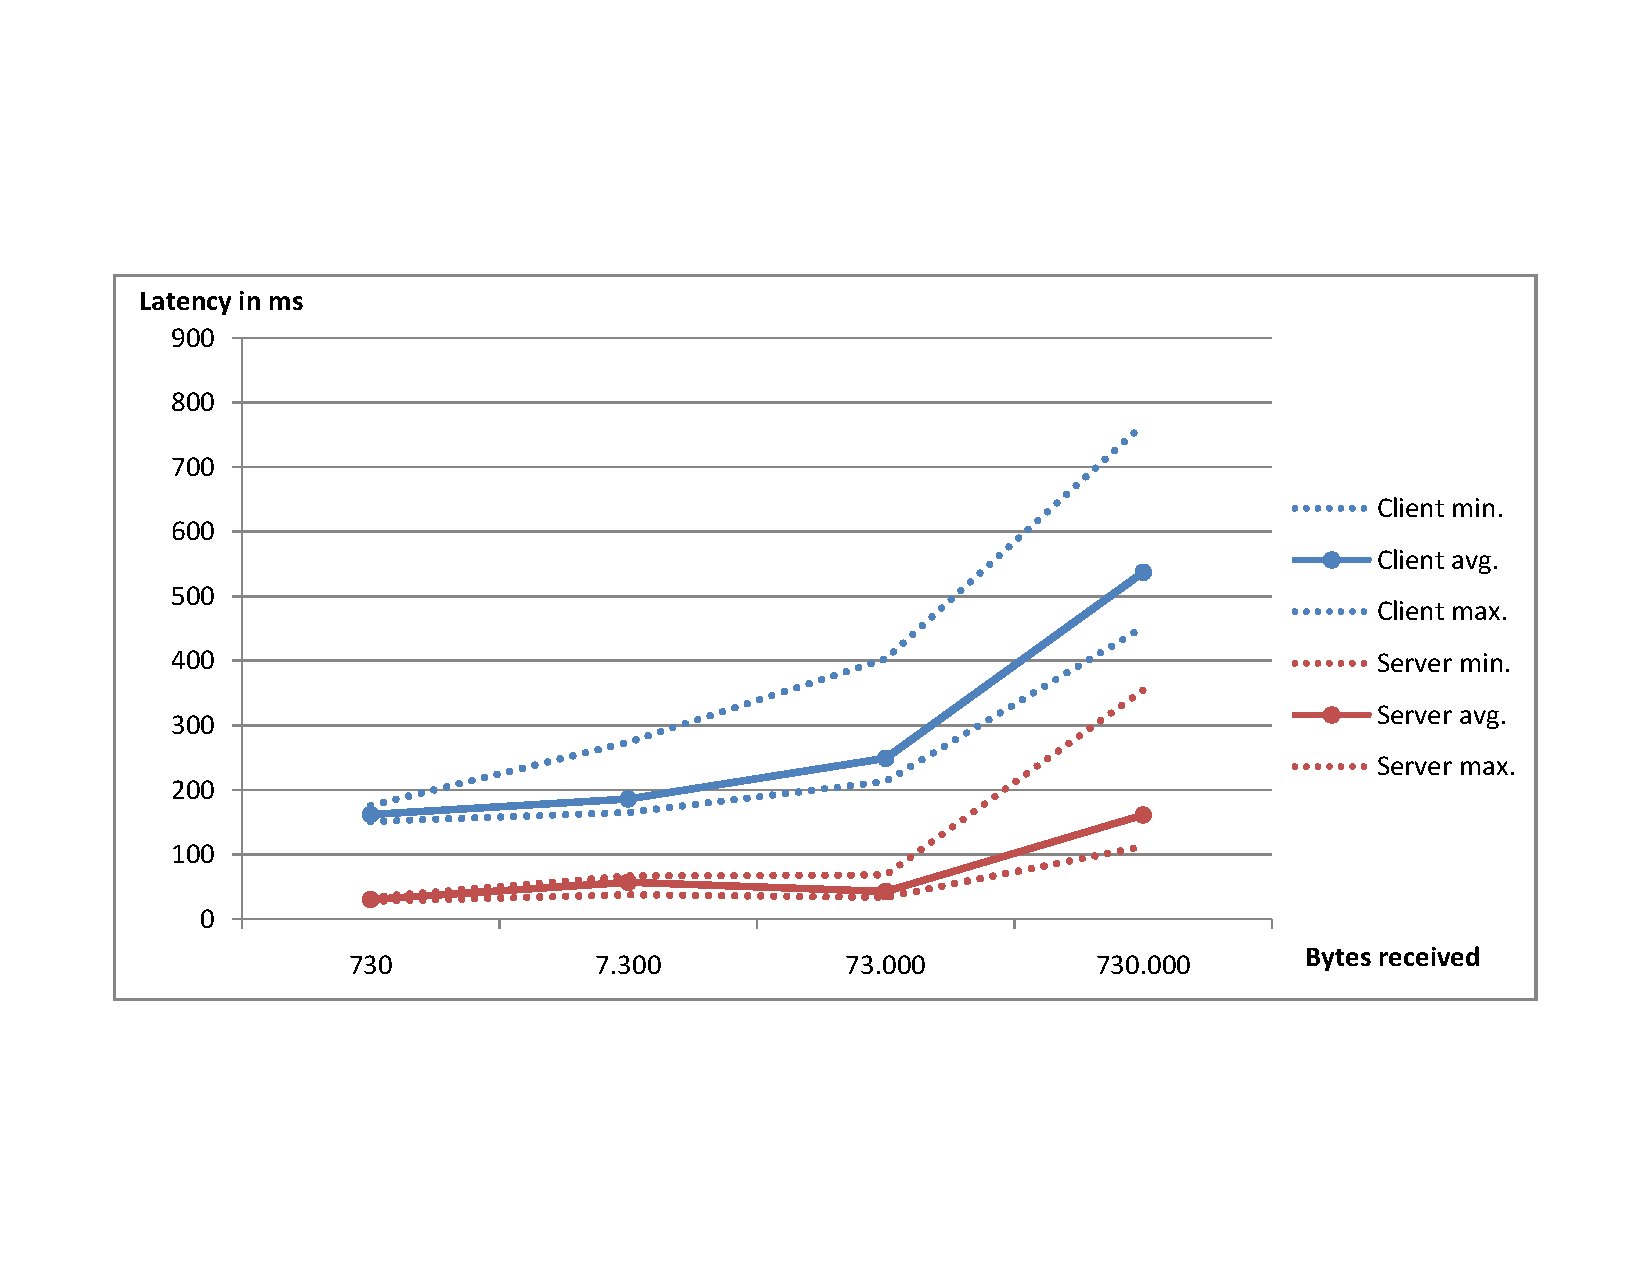
\includegraphics[trim=5cm 4cm 5cm 5cm,width=10cm]{./figures/get_obj.pdf}
\caption{Receiving Objects of Variable Size. \label{get-obj-size}}
\end{center}
\end{figure}

\begin{figure} %[placement] where placement is h,t,b,p
\begin{center}
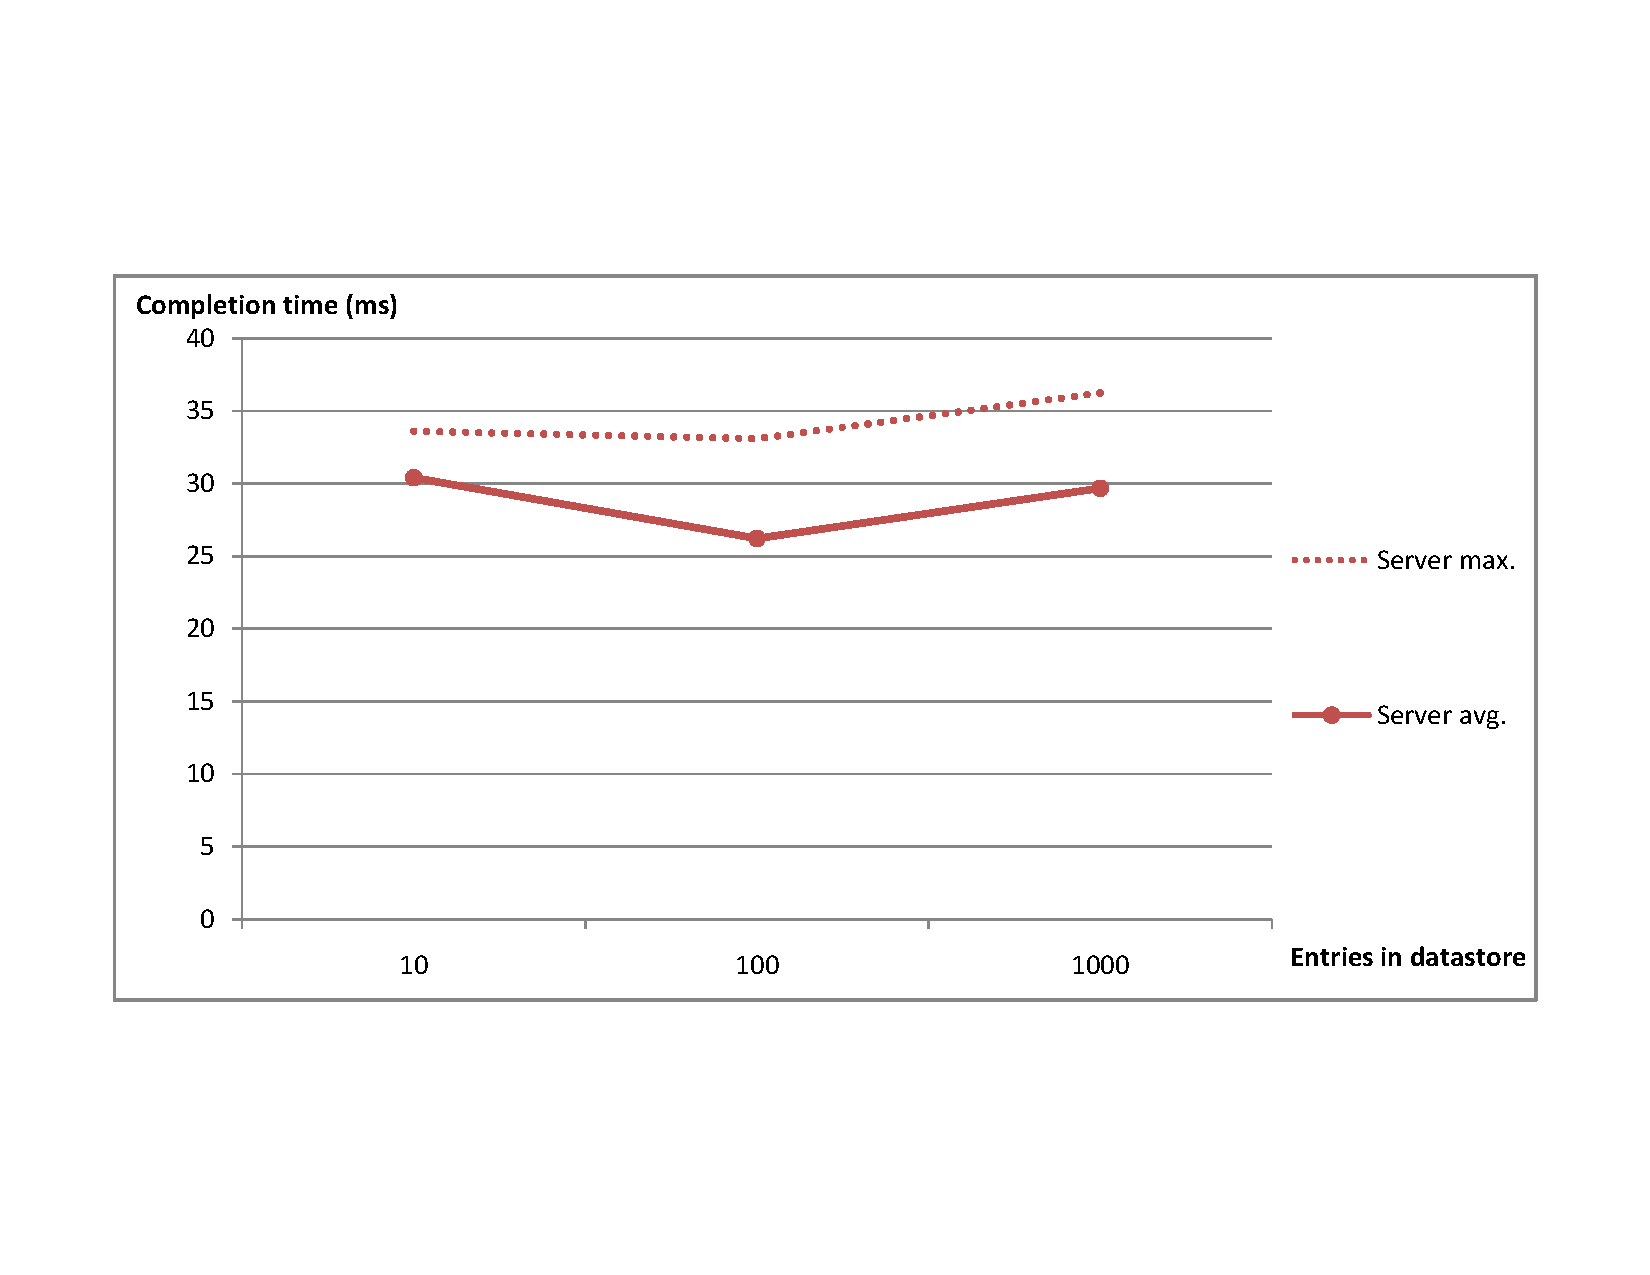
\includegraphics[trim=5cm 4cm 5cm 5cm,width=10cm]{./figures/get_amt.pdf}
\caption{Receiving Objects With Different Amounts in Datastore.
\label{get-obj-amt}}
\end{center}
\end{figure}
 
\subsubsection{Delete}
Deleting an item from the datastore should not be an issue at the client side
(the client sends the pathname of the object to be deleted, and \texttt{OK} or
\texttt{Not Found} is returned accordingly). Hence, we only measured the
\texttt{delete()} function at the server side (for results, see Figure
\ref{del-obj-amt}). Again, the server-side completion time remains the same.
 
\begin{figure} %[placement] where placement is h,t,b,p
\begin{center}
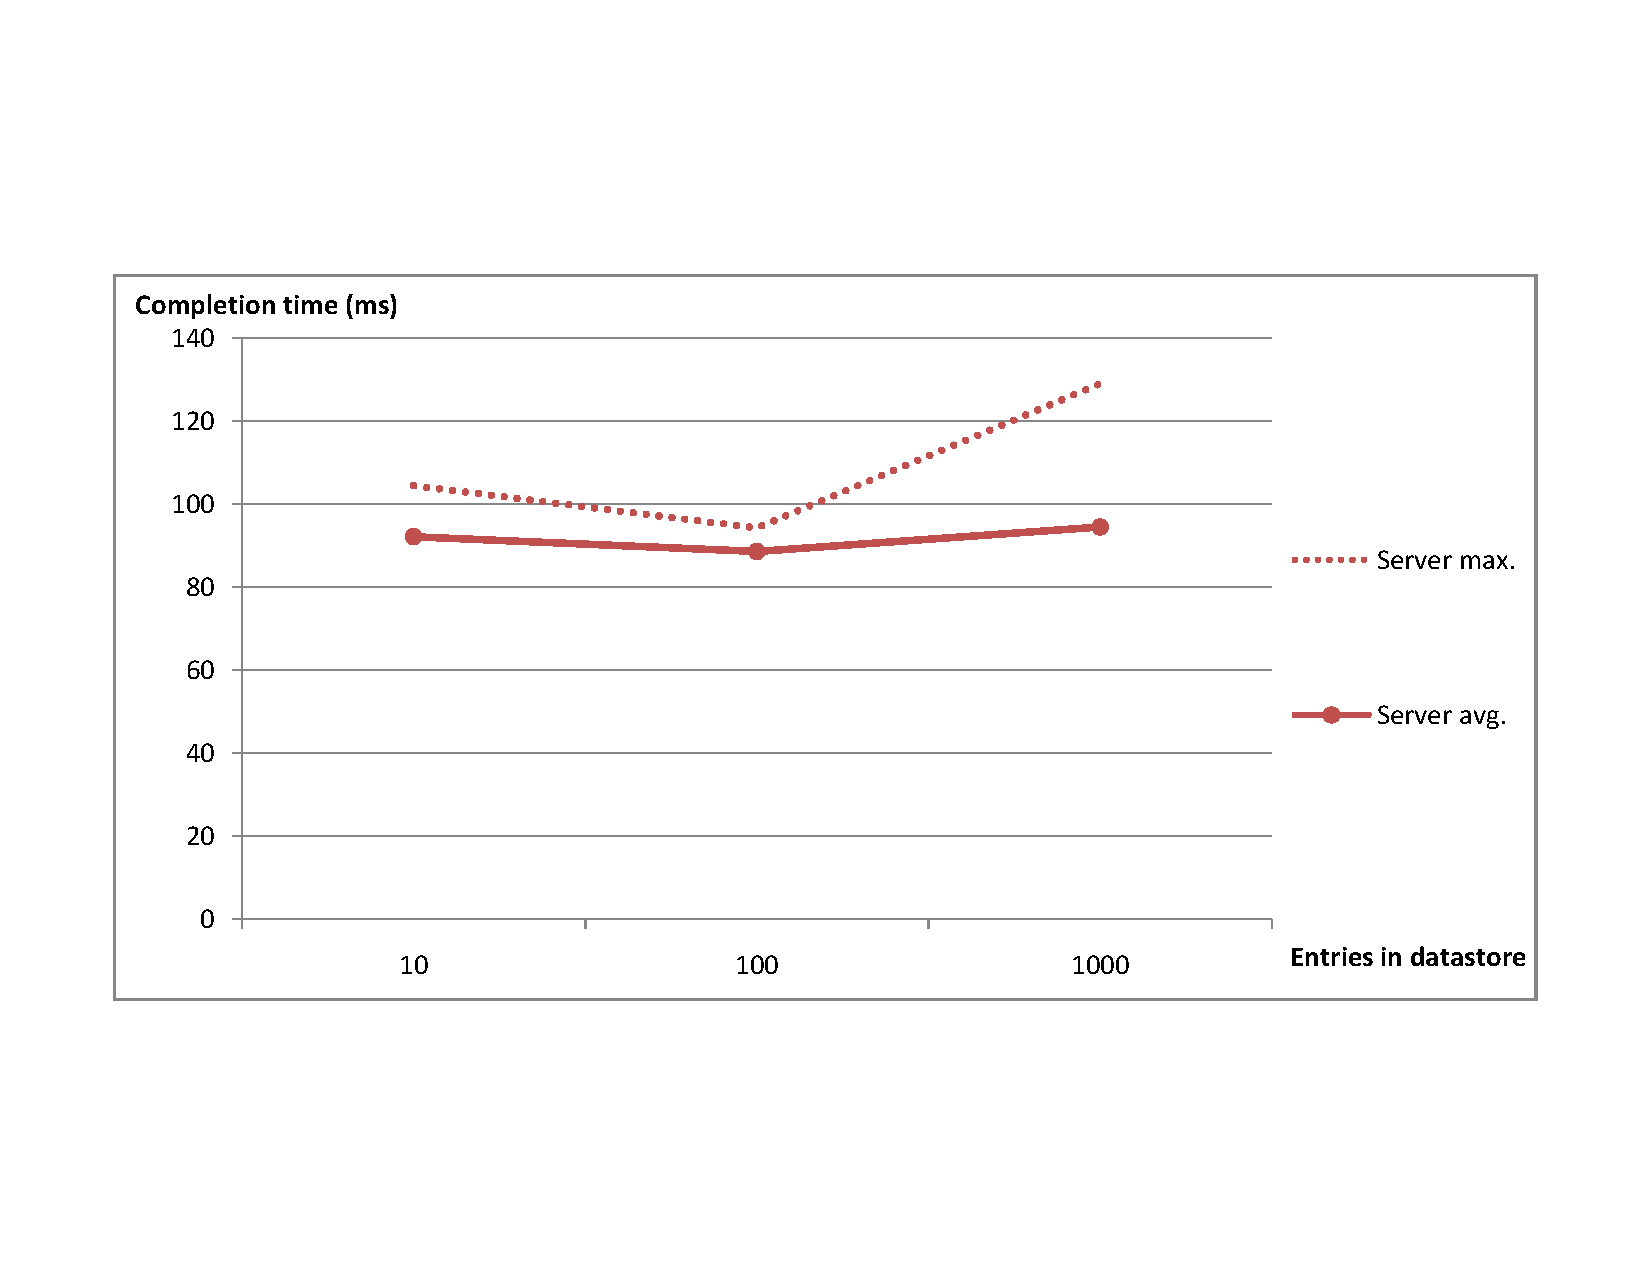
\includegraphics[trim=5cm 4cm 5cm 5cm,width=10cm]{./figures/del_amt.pdf}
\caption{Deleting Objects With Different Amounts in Datastore.
\label{del-obj-amt}}
\end{center}
\end{figure}
 
\subsubsection{Find}
Finally, an interesting function to benchmark is the find function, which is the
most compresehensive function, as stated in Section \ref{serverimpl-find}. In
Figure \ref{find-md-amt} we show some measure points we obtained from comparing
various number of key-value pairs to various number of key-value pairs present in
the datastore.

\begin{figure} %[placement] where placement is h,t,b,p
\begin{center}
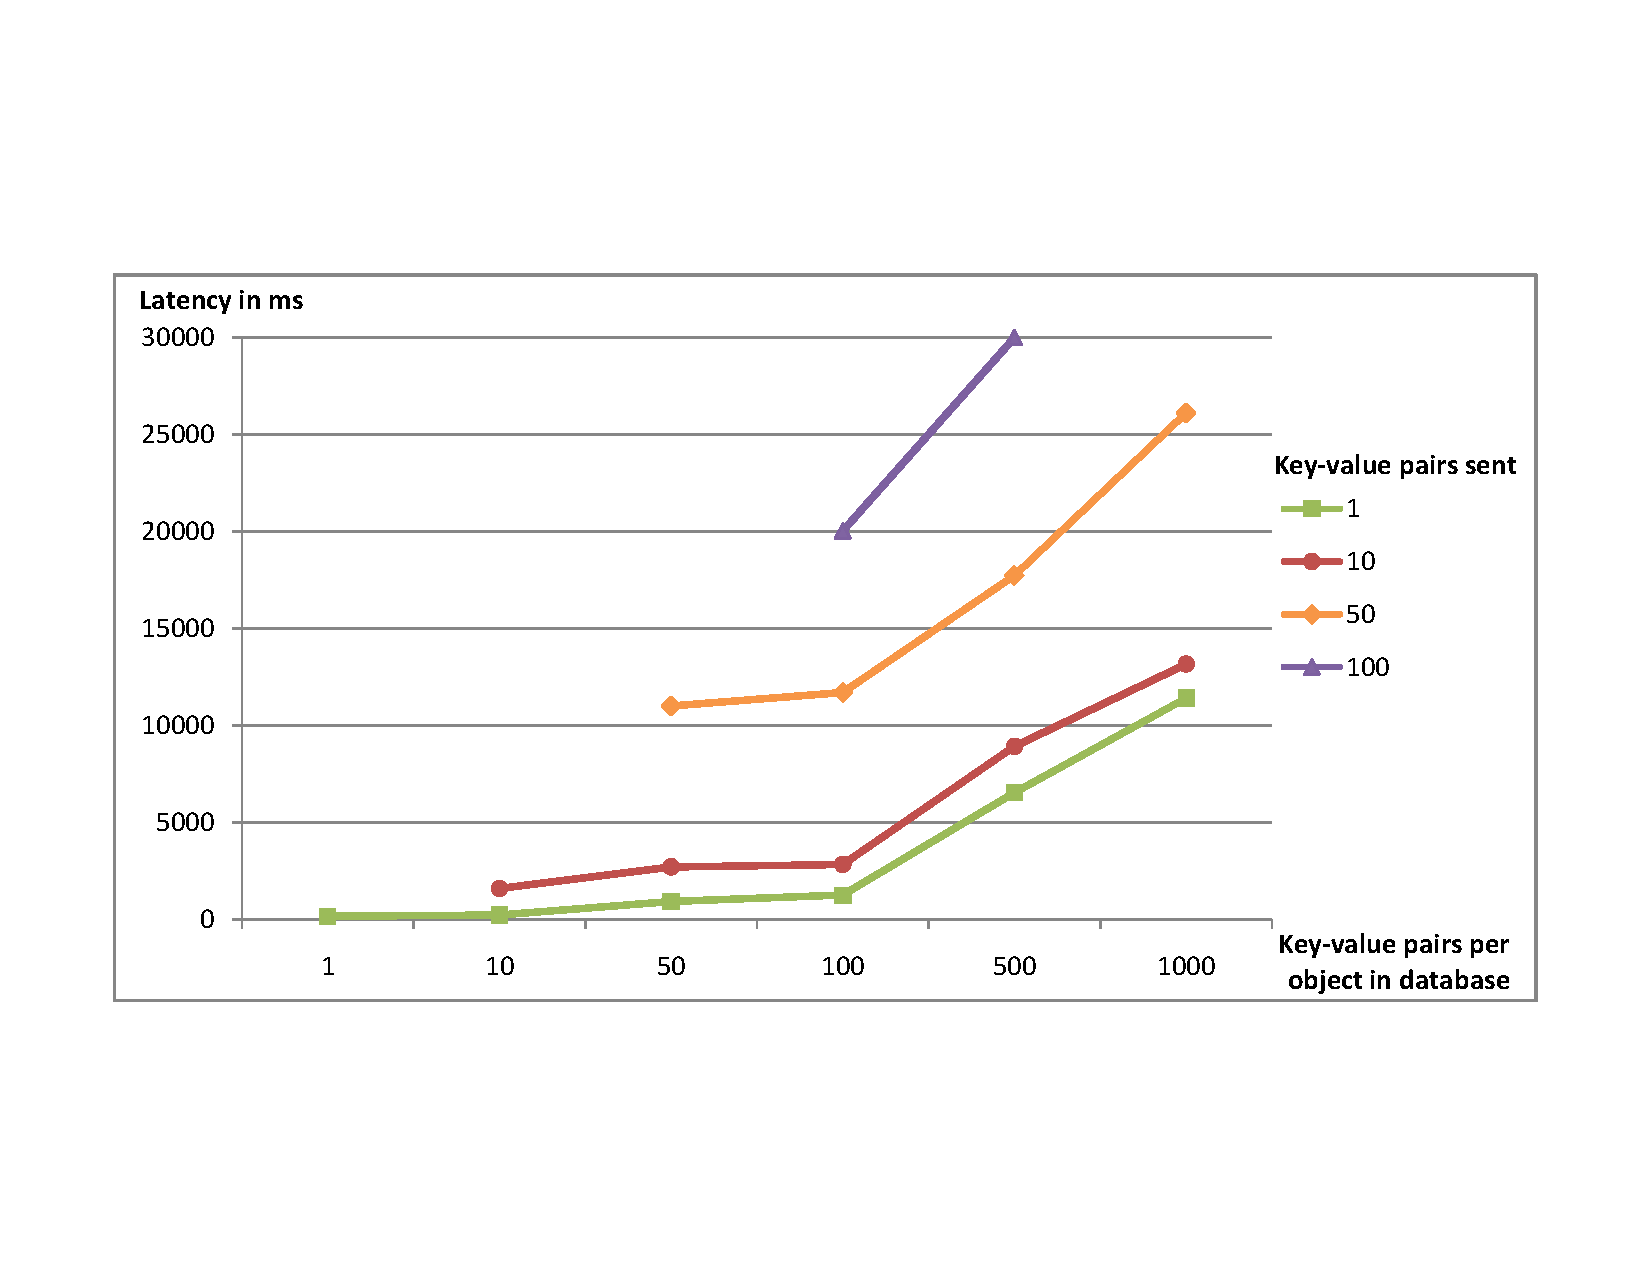
\includegraphics[trim=5cm 4cm 5cm 5cm,width=10cm]{./figures/find_amt.pdf}
\caption{Finding Meta Data With Different Amounts in Datastore.
\label{find-md-amt}}
\end{center}
\end{figure}

As we can see from Figure \ref{find-md-amt}, the completion time does increase
exponentially. For some measuring points the data points are beyond 30\,seconds
completion time, which means we received a timeout from Google. Note that we had
ten objects in the database at all time, which means we effectively had ten times
as much data to compare as suggested by the $x$-axis of the graph.

\subsection{Bandwidth}
First of all, we measured the round-trip delay, being to be 120\,ms on average.
Next we measured the upload bandwidth, by sending 5\,MB to the App Engine, which
takes 3.7\,seconds on average. Finally, we measured the download bandwidth
(client-side), by receiving 10\,MB. This gives us a round-trip delay of
26.4\,seconds on average. To let the server generate a 10\,MB response, it has to
read 10\,MB of data from a file, which has a little overhead (approximately
130\,ms).
 
Using these results, we can calculate our bandwidth in kB/sec. This is done by
substracting the round-trip delay from the upload and download round-trip delays
measured, and then divide the number of bytes sent by the number of seconds.
We can conclude that our upload bandwidth is 1360\,kB/sec, and our download
bandwidth is 372\,kB/sec.

\subsection{Parellel Benchmarks}
The results of our parallel benchmarks can be found in Figure
\ref{benchmarks-parallel-fig}. First of all we would like to state that when
connecting with 75 clients or more in parallel, the App Engine often generates a
\emph{Quota Temporarily Exceeded} error. Also, calling the ClientLogin function
shows this behavior, once we try to connect with more than 75 (identical) clients
to the App Server.
 
\begin{figure} %[placement] where placement is h,t,b,p
\begin{center}
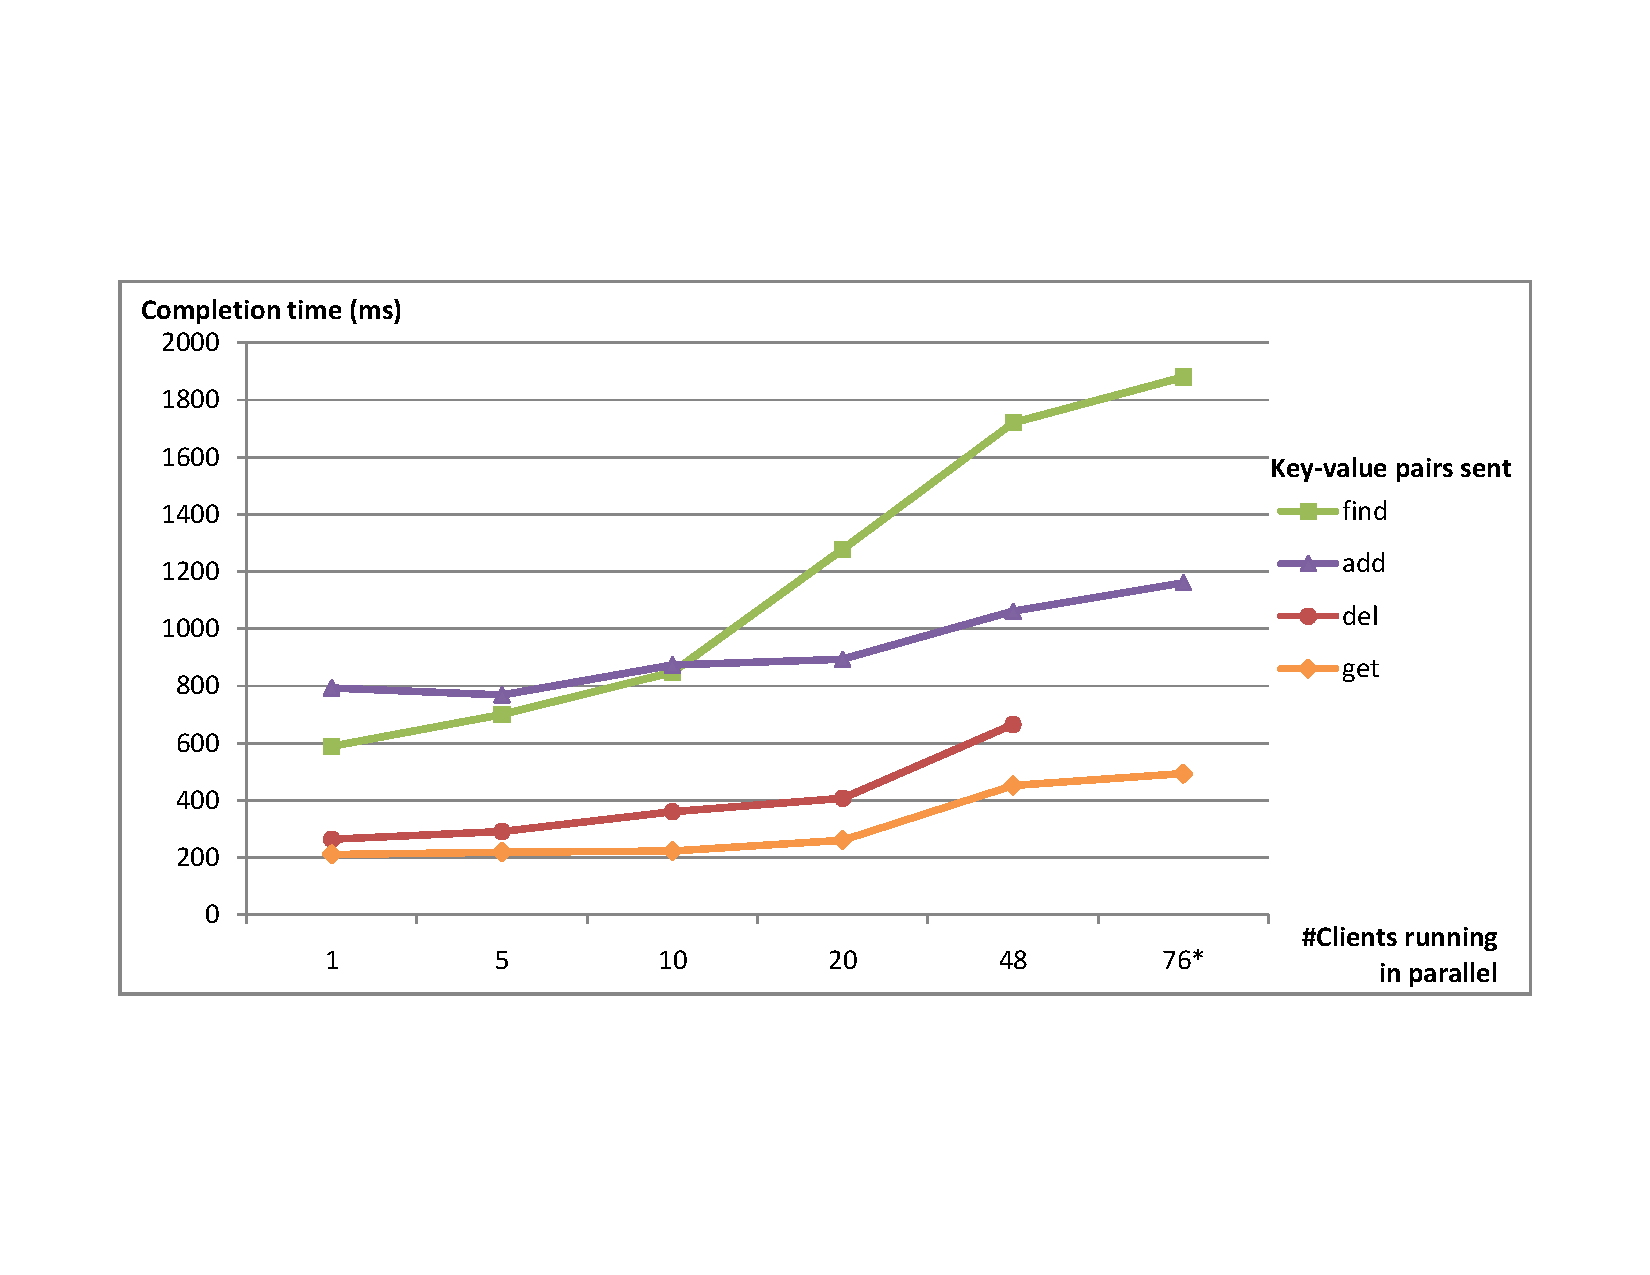
\includegraphics[trim=5cm 4cm 5cm 5cm,width=10cm]{./figures/parallel.pdf}
\caption{Connecting to the App Engine Using a Various Number of Clients in
Parallel. \label{benchmarks-parallel-fig}}
\end{center}
\end{figure}
 
As we can see, the completion time does increase if more clients connect in
parallel, but not significantly. If 75 clients would connect in parallel, the
completion only increases by 300\,ms on average. This can be explained by the
fact that Google needs to replicate our application in order to handle all the
requests, hence a delay in response time. The only exception is the
\texttt{find()} function, of which its completion time triples if 75 clients
connect in parallel, compared to 1 client. This is probably because the
\texttt{find()} function is the most complex function we benchmarked.

\subsection{Summary}
As we can conclude from our benchmark results, Google applies some restrictions
for connecting to the App Engine. The most obvious one is that the
server response time cannot be over 30\,seconds (which is stated in the App
Engine Documentation \cite{app-engine-quotas}). More subtle restrictions we
discovered whilst benchmarking our application are that quota temporarily exceeds
with requests larger than 5\,MB, or when multiple clients, connecting
simultaneously, generate enough traffic to reach the 5\,MB per minute limit.
In addition, no more than 100 clients can use ClientLogin simultaneously (i.e.
within a 60 second time span). Finally, no more than 500 data items can be
manipulated in one call. Adding over 500 data items to the datastore -- in one
call -- is possible, but removing them all at once is not.

Second thing we found is that completion time increases (both client and server
side) if the number of data sent or requested increases. Completion time also
increases if the number of clients connecting increases. However, when there is
more data present in the datastore (i.e. more data items to be searched from),
the completion time does not increase.

Finally, we suspect Google from limiting the download bandwidth, since there is
a significant difference between upload and download speed.
